
\documentclass[10pt,landscape]{scrartcl}

\usepackage[english]{babel}
% \usepackage[ngerman]{babel}
\usepackage[utf8]{inputenc}

\usepackage{lmodern}

\usepackage{ifthen}

\usepackage{graphicx}
% \usepackage{pstricks}
% \usepackage{relsize}
% \usepackage[decimalsymbol=comma,exponent-product = \cdot, per=frac]{siunitx}
% \sisetup{range-phrase=\,bis\,}

\usepackage{xargs}
\usepackage{calc}
\usepackage{amsmath}
\usepackage{amsfonts}
\usepackage{mathtools}
\usepackage{amssymb}

\usepackage{cancel}
\usepackage{trfsigns}
\usepackage{array}
\usepackage{enumerate}
\usepackage{enumitem}

\usepackage{caption}
\usepackage{subcaption}

\usepackage{multicol}

\usepackage{pdflscape}
\usepackage[table]{xcolor}

\usepackage{float}

%%%%%%%%%%%%%%%%%%%%%%%%%%%%%%%%%%%%%%%%%%%%%%%%%%%%%%%%%%%%%%%%%%%%%%%%%%%%%%%%
\newboolean{WITHPSTRICKS}
\setboolean{WITHPSTRICKS}{false}


\newcommand{\PROFESSOR}{Prof.\ Dr.\ Thomas Carraro}
\newcommand{\ASSISTANT}{\setlength{\tabcolsep}{0pt}\begin{tabular}{l} Dr. Ulrike Kochan-Eilers\end{tabular}}

\newcommand{\Jahr}{2025}
% \newcommand{\Trimester}{HT}
\newcommand{\Trimester}{FT}
\newcommand{\Kurs}{Mathematik III/C (WI/ET)}
\newcommand{\TYPE}{Aufgabenblatt}
\newcommand{\BLATT}{4}
\newcommand{\TOPIC}{lineare Dgl. 1.Ordnung, lineare Dgl. h\"oherer Ordnung}
\usepackage{pstricks}
\usepackage{pst-plot}
\usepackage{circuitikz}
%%%%%%%%%%%%%%%%%%%%%%%%%%%%%%%%%%%%%%%%%%%%%%%%%%%%%%%%%%%%%%%%%%%%%%%%%%%%%%%%
\newboolean{mitLoes}
\setboolean{mitLoes}{false}
%\setboolean{mitLoes}{true}

%%%%%%%%%%%%%%%%%%%%%%%%%%%%%%%%%%%%%%%%%%%%%%%%%%%%%%%%%%%%%%%%%%%%%%%%%%%%%%%%


%\setboolean{WITHPSTRICKS}{false}
%\setboolean{WITHPSTRICKS}{true}


\usepackage{tikz}
\usetikzlibrary{arrows,automata,backgrounds,calendar,decorations.pathmorphing,fadings,shadings,calc,intersections}
\usetikzlibrary{decorations.pathreplacing}
\usetikzlibrary{decorations.shapes}
\usetikzlibrary{decorations.footprints}
\usetikzlibrary{decorations.text}
\usetikzlibrary{positioning}
\usetikzlibrary{through}
\usepackage[utf8]{inputenc}


\ifthenelse{\boolean{WITHPSTRICKS}}{%
\usepackage{auto-pst-pdf}
\usepackage{pstricks,pst-plot,pst-text}
}{}

\usepackage{pgfplots}

%%%%%%%%%%%%%%%%%%%%%%%%%%%%%%%%%%%%%%%%%%%%%%%%%%%%%%%%%%%%%%%%%%%%%%%%%%%%%%%%
\usepackage{mbdefAufgaben}

%%%%%%%%%%%%%%%%%%%%%%%%%%%%%%%%%%%%%%%%%%%%%%%%%%%%%%%%%%%%%%%%%%%%%%%%%%%%%%%%
\newboolean{mitErg}
%\setboolean{mitErg}{false}

%%%%%%%%%%%%%%%%%%%%%%%%%%%%%%%%%%%%%%%%%%%%%%%%%%%%%%%%%%%%%%%%%%%%%%%%%%%%%%%%
\newcounter{Aufg}
\setcounter{Aufg}{0}
\newcounter{Blatt}
\setcounter{Blatt}{1}

%%%%%%%%%%%%%%%%%%%%%%%%%%%%%%%%%%%%%%%%%%%%%%%%%%%%%%%%%%%%%%%%%%%%%%%%%%%%%%%%
%\usepackage{KopfEnglish}

% Seitenraender
%\textwidth = 285mm
%\textheight = 180mm
%\leftmargin 5mm
%\oddsidemargin = -20mm
%\evensidemargin = -20mm
%\topmargin = -25mm
%\parindent 0cm
%\columnsep 2cm

% % % Aufgabenstellung
% % % Schwierungkeitsgrad mit "e" , "f" oder "v" angeben
% % % "e" Einführung   
% % % "f" Festigung
% % % "v" Vertiefung  

\newcommand{\Aufgabe}[3][]{
\stepcounter{Aufg}
\subsubsection*{Aufgabe 
\arabic{Aufg}\ifthenelse{\equal{#1}{e}}{}{\ifthenelse{\equal{#1}{f}}{
$\!\!{}^\star$}{\ifthenelse{\equal{#1}{v}}{$^{\star\star}$}{}}}{: #2}}
{#3}
}
% % % Ergebnisse jeweils am Ende des Aufgabenblattes Anzeigen
\newcommand{\Ergebnisse}{}
\makeatletter
\newcommand{\Ergebnis}[1]{
	\g@addto@macro{\Ergebnisse}{#1}
}
\makeatother
\makeatletter
\newcommand{\ErgebnisC}[2]{
\@ifundefined{c@#1}
{\newcounter{#1}}
{}
\setcounter{#1}{\theAufg}

\ifthenelse{\boolean{mitErg}}{	\g@addto@macro{\Ergebnisse}{\subsubsection*{Ergebnisse zu Aufgabe \arabic{#1}:}
}%
	\g@addto@macro{\Ergebnisse}{#2}}{}
}
\makeatother


% % % Lösungen
\newcommand{\Loesung}[1]{
	\ifthenelse{\boolean{mitLoes}}
	{\subsubsection*{Lösung \arabic{Aufg}:}
		#1}
	{}
}
% % % % % % % % % % % % % % % % % % % % % % % % % % % % % % % % % % % % % % % % % % % % % % % % % % % % % %
% % % % % % % % % % % % % % % % % % % % % % % % % % % % % % % % % % % % % % % % % % % % % % % % % % % % % %
% % % % % % % % % % % % % % % % % % % % % % % % % % % % % % % % % % % % % % % % % % % % % % % % % % % % % %
\begin{document}
%\begin{twocolumn}
% % % % % % % % % % % % % % % % % % % % % % % % % % %

%%%%%%%%%%%%%%%%%%%%%%%%%%%%%%%%%%%%%%%%%%%%%%%%%%%%%%%%%%%%%%%%%%%%%%%%%%%%%%%%
% Set the TITLE of the sheet here:
%\uebheader{\Kurs}{\arabic{Blatt}}{\Trimester\,\Jahr}{\TOPIC}
%\uebheader{\Kurs}{\arabic{Blatt}}{\Trimester\,\Jahr}{\TOPIC}
%\uebheader{\Kurs}{\arabic{Blatt}}{\Trimester\,\Jahr}{\TOPIC}
%\ruleBig

\setboolean{mitErg}{false}
\setboolean{mitErg}{true}


%%%%%%%%%%%%%%%%%%%%%%%%%%%%%%%%%%%%%%%%%%%%%%%%%%%%%%%%%%%%%%%%%%%%%%%%%%%%%%%%
% Set the INTRODUCTION section of the sheet here:
% \input{introduction.tex}

\textbf{Einführende Bemerkungen}

\begin{itemize}
\item Vermeiden Sie die Verwendung von Taschenrechnern oder Online-Ressourcen.
% \item Die mit einem Stern *) markierten (Teil-)Aufgaben entfallen in diesem Trimester. Stattdessen werden einzelne Online-Aufgaben im ILIAS-Kurs kenntlich gemacht, zu denen Sie dort Ihre L\"osungswege zur Korrektur hochladen k\"onnen. 
% \item Die mit zwei Sternen  **) markierten (Teil-)Aufgaben richten sich an Studierende, die die \"ubrigen Aufgaben bereits gel\"ost haben und die Inhalte weiter vertiefen m\"ochten. 
\end{itemize}

\ruleBig

%Mathe III Blatt 4


\Aufgabe[e]{LR-Kreis}
{
Ein Stromkreis habe einen Widerstand von \ $R=0.8$ Ohm \ und eine Selbstinduktion von \ $L=4$ Henry\,. Bis zur Zeit \ $t_0=0$ \ fließe kein Strom. Dann wird eine Spannung von \ $U=5$ Volt \ angelegt. Nach $5$ Sekunden wird
die Spannung abgeschaltet. Berechnen Sie den Stromverlauf \
$I(t)$ \ für \ $0 \le t \le 5$ \ und \ $t > 5$. \\ 
\textbf{Hinweis}: In diesem Stromkreis gilt $L\dot I(t) + RI(t)=U(t)$
}

\Loesung{
Es gilt gilt die Differentialgleichung
\[
  L\dot{I}(t)+RI(t)=U(t)
\]

Für \ $0\leq t\leq 5$ \ gilt \ $U(t)=5$\,. Die Trennung der Variablen führt zu
\[
  \int \frac{dI}{U-R I}=\int \frac{1}{L} \,dt,\Rightarrow
   -\frac{1}{R}\ln | U-RI(t)| =\frac{1}{L}t + c_1\,, \;\;    c_1 \in \R\,. 
\]
Auflösen nach $I(t)$ liefert (mit $c_2=\EH{c_1}$)
\[
  U-RI(t)=c_2 e^{-Rt/L}
\] 
und somit
$$
   I(t)=\frac{1}{R} \big( U-c_2 e^{-Rt/L} \big)\,.
$$

Einsetzen der Anfangsbedingung \ $I(0)=0$ \ ergibt \ $c_2=U$ \ und
$$
  I(t)=\frac{U}{R}\big(1-e^{-R/Lt}\big)\,.
$$
Einsetzen der gegebenen Zahlenwerte ergibt die Lösung
$$ 
  I(t) = 6.25\, \big(1-e^{-0.2 t}\big) \text{ f\"ur } 0 < t < 5\,. 
$$


Im Zeitraum \ $t>5$ \ ist $U(t)=0$ \ und der Anfangsstrom ist
$$
I(5)=I_0=6.25\,\big(1-e^{-1}\big)\ .
$$
Die Lösung der Differentialgleichung ist
$$
  \int \frac{dI}{I}=-\int\limits \frac{R}{L}dt\Rightarrow  \ln |I(t)|=-\frac{R}{L}t+c_3
$$ 
und damit
$$
  I(t)= c_4 e^{-Rt/L}\ .$$
Aus \ $I(t_0)=I_0$ \ folgt 
$$
 I(t) = I_0 e^{-R(t-t_0)/L}\ .
$$
Einsetzen der Zahlenwerte ergibt die Lösung 
$$ 
I(t) = 6.25 \big(1-e^{-1}\big) e^{-0.2 (t-5)} \text{ f\"ur } t > 5\ . 
$$
}


\ErgebnisC{gewdglStrmLrkr001}{
$I(t)=\left\{\begin{array}{ll}
6.25\, \big(1-e^{-0.2 t}\big)& \text{ f\"ur } 0 < t < 5\\
6.25 \big(1-e^{-1}\big) e^{-0.2 (t-5)}& \text{ f\"ur } t > 5
\end{array}\right.$
}

\ifthenelse{\boolean{mitLoes}}{\ruleBig \cleardoublepage}{}

\Aufgabe[e]{Anfangswertproblem}
{
Gegeben ist die Differentialgleichung
$$
y'(x)+y(x)\sin(x)=\sin(2x).
$$

\begin{abc}
\item Bestimmen Sie die allgemeine L\"osung.
\item Bestimmen Sie die L\"osung f\"ur den Anfangswert $y(0)=1$.
\end{abc}

}

\Loesung{
\begin{abc}
\item Wir l\"osen zun\"achst die hom. lin. Dgl. mit Trennung der Variablen:
\begin{align*}
y'+y\sin(x)=0 & \Rightarrow  \int \frac{\mathrm{d}y}{y} =  \int - \sin(x) \mathrm{d}x  \\
              & \Rightarrow \ln|y(x)| = \cos(x) + \tilde{C} \\
              & \Rightarrow |y(x)| = e^{\tilde{C}} e^{\cos(x)} \\
              & \Rightarrow y(x) = \pm e^{\tilde{C}} e^{\cos(x)}
\end{align*}
Die allgemeine hom. L\"osung lautet:
$$
y_{\text{h}}(x) =  C e^{\cos(x)}.
$$
Zur Bestimmung der speziellen L\"osung der inhom. Dgl. verwenden wir den Produktansatz:
$$
y(x) = c(x) e^{\cos(x)} \Rightarrow y'(x) = c'(x) e^{\cos(x)}-c \sin(x) e^{\cos(x)}.
$$
Einsetzen in die Dgl. ergibt:
$$
c'(x) e^{\cos(x)}  -c \sin(x) e^{\cos(x)} +c e^{\cos(x)} \sin(x) = \sin(2x)
$$
$$
\Rightarrow c'(x) = \sin(2x)  e^{-\cos(x)}.
$$
Um $c(x)$ zu bestimmen wird die Trennung der Variablen durchgef\"uhrt:
$$
\int \mathrm{d}C = \int \sin(2x)  e^{-\cos(x)}  \mathrm{d}x = \int 2 \cos(x)\sin(x)e^{-\cos(x)}   \mathrm{d}x.
$$
Das rechte Integral l\"asst sich mit Substitution l\"osen:
$$
\Rightarrow c(x) = (2\cos(x)+2) e^{-\cos(x)}.
$$
Damit ist die partikul\"are L\"osung:
$$
y_{\text{p}}(x) = c(x) e^{\cos(x)} = 2\cos(x)+2.
$$
Die allgemeine L\"osung der Dgl. ist damit
$$
y(x) = C  e^{\cos(x)} +2\cos(x)+2.
$$

\item 
$$
y(0)=1 = C e^{\cos(1)}+2\cos(1)+2
$$
$$
\Rightarrow C = (-1-2\cos(1))e^{-\cos(1)}
$$
Einsetzen in die allgemeine L\"osung ergibt
$$
y(x) = -3 e^{\cos(x)-1}+2\cos(x)+2.
$$
\end{abc}
}


\ErgebnisC{gewdgl_Anfangswertproblem03}{
\begin{abc}
\item $y(x) = C  e^{\cos(x)} +2\cos(x)+2$
\item $y(x) = -3 e^{\cos(x)-1}+2\cos(x)+2$

\end{abc}
}


\ifthenelse{\boolean{mitLoes}}{\ruleBig \cleardoublepage}{}

\Aufgabe[e]{Trennung der Veränderlichen und Anfangswertproblem}

{
Klassifizeren die folgende Differentialgleichung und bestimmen Sie die Lösung des Anfangswertproblems mit $y(0) = 0$ und $y'(0) = 6$:
 $$
 y''(x) - 2 y'(x) - 3y(x) = 0.
 $$
}

\Loesung{
Die Nullstellen des charakteristischen Polynoms
$p(\lambda)=\lambda^2-2\lambda-3$ sind $\lambda_1=-1$ und $\lambda_2=3$.

Die allgemeine Lösung ist
$$ y(x) = c_1 \operatorname{e}^{-x} + c_2 \operatorname{e}^{3x}  \text{ mit } c_1,c_2 \in \mathbb{R} .$$

Mit den Anfangswertbedingungen $y(0)=c_1 + c_2 \stackrel{!}{=} 0$ und 
$y^\prime(0) = -c_1 + 3c_2 \stackrel{!}{=} 6$ erhalten wir das lineare System
% $$ \begin{array}{rcrl}
$$ \begin{array}{rcrl}
   c_1 & + & c_2 & = 0, \\
  -c_1 & + & 3c_2 & = 6 
   \end{array} $$
mit Lösung $c_2=3/2$ und $c_1=-3/2$. Damit ist 
$$ y(x) = -\frac32  \operatorname{e}^{-x} + \frac32 \operatorname{e}^{3x}. $$
%    \end{array} $$
% with solution $c_2=3/2$ and $c_1=-3/2$. This yields
% $$ y(x) = -\frac32  \operatorname{e}^{-x} + \frac32 \operatorname{e}^{3x}. $$

}


\ifthenelse{\boolean{mitLoes}}{\ruleBig \cleardoublepage}{}

\Aufgabe[e]{Homogene lineare Differentialgleichungen}
{
Bestimmen Sie die allgemeine Lösung der folgenden linearen Differentialgleichungen
\begin{abc}
\item $y'' - y = 0$, 
\item $y''' + y'' = 0$, 
\item $y''+y'-2y = 0$, 
\item $y''+y = 0$.
\end{abc}
}

\Loesung{
\begin{abc}
\item 
Wir lösen die homogene Gleichung
$$
y'' -y = 0.
$$
Das charakteristische Polynom ist
$$
\lambda^2 -1 = 0
$$
mit den Nullstellen $\lambda_1 = 1$ und $\lambda_2 = -1$.
Damit ist die allgemein L\"osung der homogenen Dgl.
$$
y_h = c_1 \operatorname{e}^x + c_2 \operatorname{e}^{-x}.
$$

\item
Wir lösen die homogene Gleichung
$$
y''' + y'' = 0.
$$
Das charakteristische Polynom ist
$$
\lambda^3 + \lambda^2 = \lambda^2(\lambda +1)= 0
$$
mit der doppelten Nullstelle $\lambda = 0$ und der einfachen Nullstelle $\lambda = -1$.
Damit ist die homogene Lösung
$$
y_h = (c_1+c_2x)+ c_3\operatorname{e}^{-x}.
$$

\item
Wir lösen homogene Gleichung
$$
y''+y'-2y = 0.
$$
Das charakteristische Polynom ist
$$
\lambda^2 + \lambda -2 = 0
$$
mit den Nullstellen $\lambda_1 = -2$ und $\lambda_2 = 1$.
Damit ist die homogene Lösung
$$
y_h = c_1 \operatorname{e}^{-2x} + c_2 \operatorname{e}^x.
$$

\item
Wir lösen die homogene Gleichung
$$
y'' + y = 0
$$
mit dem charakteristischen Polynom
$$
\lambda^2 + 1 = 0.
$$
Die Nullstellen sind $\lambda = \pm \operatorname{i}$
Damit ist die homogene Lösung
$$
y_h = c_1 \cos(x) + c_2\sin(x).
$$

\end{abc}
}


\ErgebnisC{oderesonanz001}{
\begin{abc}
\item $y(x)= c_1 \operatorname{e}^x + c_2 \operatorname{e}^{-x} $
\item $y(x)= (c_1+c_2x)+ c_3\operatorname{e}^{-x} $
\item $y(x)= c_1 \operatorname{e}^{-2x} + c_2 \operatorname{e}^x $
\item $y(x)= c_1 \cos(x) + c_2\sin(x) $
\end{abc}
}

\ifthenelse{\boolean{mitLoes}}{\ruleBig \cleardoublepage}{}

%\Aufgabe[e]{Komplexe Nullstellen des charakteristischen Problems}
{
Bestimmen Sie die Lösung der folgenden Differentialgleichung:
% Determine the solution of the following differential equation:
$$y^{\prime\prime}+4y^\prime+5y=0$$
}

\Loesung{

Das charakteristische Polynom $p(\lambda)=\lambda^2+4\lambda+5$ hat die Nullstellen
$$\lambda_1=-2+i, \lambda_2=-2-i$$
die Lösung ist dann
\begin{align*}
y&=C_1\EH{-2t+\imag t}+C_2\EH{-2t-\imag t}\\
&= \EH{-2t}(C_1(\cos t+\imag \sin t)+C_2(\cos t-\imag \sin t)) \\
&= \EH{-2t}(c_1\cos t+c_2 \sin t ),
\end{align*}
wobei $c_1=C_1+C_2$ und $c_2 = i(C_1-C_2)$ die reellen Konstanten sind. \\
Die komplexen Konstanten können durch die reellen Konstanten wie folgt ausgedrückt werden:
$C_1=\overline{C_2}=\dfrac{c_1-\imag c_2}{2}$.
}


\ErgebnisC{AufggewdglLinenOrd004}
{
$y(x) = \EH{-2t}(c_1\cos t+c_2 \sin t )$
}


%\ifthenelse{\boolean{mitLoes}}{\ruleBig \cleardoublepage}{}

\Aufgabe[e]{Harmonischer Oszillator}
{\label{aufgabe:oszillator}
Man betrachte die Differentialgleichung
\[
y'' + 2\rho y' + \omega^2 y = 0, \quad \text{mit } \rho, \omega \in \mathbb R_+
\]
Die gegebene Differentialgleichung, ist eine klassische Form einer linearen Differentialgleichung zweiter Ordnung mit konstanten Koeffizienten. Aus physikalischer Sicht beschreibt diese Gleichung typischerweise gedämpfte harmonische Bewegungen, wobei:
\begin{itemize}
  \item \( y(t) \) die Verschiebung des Systems vom Gleichgewicht über die Zeit darstellt.
  \item \( \rho \) (der Koeffizient der ersten Ableitung \( y' \)) repräsentiert den Dämpfungsfaktor, der beeinflusst, wie schnell das System Energie durch Reibung oder andere resistive Kräfte verliert.
  \item \( \omega^2 \) (der Koeffizient von \( y \)) steht im Zusammenhang mit der Steifigkeit des Systems oder der Kraft, die es ins Gleichgewicht zurückführt. Der Parameter \( \omega \) selbst wird oft als natürliche Frequenz des ungedämpften Systems betrachtet.
\end{itemize}

\textbf{Physikalische Interpretationen}
\begin{enumerate}
  \item \textbf{Mechanische Systeme:} In der Mechanik kann diese Gleichung ein Masse-Feder-Dämpfer-System modellieren, bei dem eine Masse an einer Feder und möglicherweise einem Dämpfungselement (wie einem Stoßdämpfer) befestigt ist. Die Masse oszilliert um eine Gleichgewichtsposition, wobei die Feder eine rückstellende Kraft proportional zur Verschiebung liefert und der Dämpfer eine Kraft proportional zur Geschwindigkeit bereitstellt, die der Bewegung entgegenwirkt.

\begin{center}
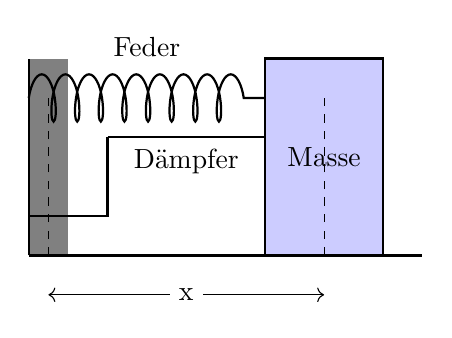
\begin{tikzpicture}
    % Draw the wall
    \fill[gray] (-1,0) rectangle (-0.5,2.5);
    \draw[thick] (-1,0) -- (-1,2.5);

    % Draw the spring
    \draw[thick,decorate,decoration={coil,aspect=0.3,segment length=3mm,amplitude=3mm}] (-1,2) -- (2,2) node[midway,above=4mm] {Feder};

    % Draw the damper
    \draw[thick] (-1,0.5) -- (0,0.5) -- (0,1.5);
    \draw[thick] (0,1.5) -- (2,1.5) node[midway,above=-6mm] {D\"ampfer};

    % Draw the mass
    \fill[blue!20!white] (2,0) rectangle (3.5,2.5);
    \draw[thick] (2,0) -- (2,2.5) -- (3.5,2.5) -- (3.5,0) -- cycle;
    \node at (2.75,1.25) {Masse};

    % Ground and vertical lines
    \draw[thick] (-1,0) -- (4,0);
    \draw[dashed] (-0.75,0) -- (-0.75,2);
    \draw[dashed] (2.75,0) -- (2.75,2);
    
    % Distance annotation
    \draw[<->] (-0.75,-0.5) -- (2.75,-0.5) node[midway,fill=white] {x};
\end{tikzpicture}
\end{center}


  \item \textbf{Elektrische Schaltkreise:} In der Elektrotechnik kann die Gleichung einen RLC-Schaltkreis (einen Schaltkreis, der einen Widerstand \( R \), eine Induktivität \( L \), und einen Kondensator \( C \) enthält) beschreiben. Hier könnte \( y(t) \) die elektrische Ladung oder den Strom darstellen, \( 2 \rho = R/L \) und \( \omega^2 = 1/(LC)\). Das Verhalten des Schaltkreises — ob er oszilliert oder schnell stabilisiert wird — hängt von den Werten dieser Komponenten ab.

\begin{center}
\begin{circuitikz}
    \draw
    % Voltage source
    (0,0) to[V, v=$V_s$, invert] (0,3)
    % Resistor
    to[R, l=$R$, v<=$V_R$] (3,3)
    % Inductor
    to[L, l=$L$, v<=$V_L$] (6,3)
    % Capacitor
    to[C, l=$C$, v<=$V_C$] (6,0)
    % Connect back to the voltage source
    -- (0,0);

    % Labels
    \node at (3,1.5) {RLC Stromkreis};
\end{circuitikz}
\end{center}
\end{enumerate}
Diese Gleichung ist allgemein bekannt als \textit{"Gedämpfter harmonischer Oszillator"} oder einfach als \textit{"Gedämpfter Oszillator"}. Sie umfasst drei spezifische Szenarien basierend auf dem Wert von \( \rho \) im Vergleich zu \( \omega \):
\begin{enumerate}
  \item \textbf{Überdämpft (\( \rho > \omega \)):} Das System kehrt ohne Oszillation langsam zum Gleichgewicht zurück.
  \item \textbf{Kritisch gedämpft (\( \rho = \omega \)):} Das System kehrt so schnell wie möglich ohne Oszillation zum Gleichgewicht zurück.
  \item \textbf{Untergedämpft (\( \rho < \omega \)):} Das System oszilliert mit einer Amplitude, die allmählich auf null abnimmt.
\end{enumerate}
\textbf{Aufgabe:}
\smallskip
Bestimmen Sie die Lösung der DGl für alle drei Fälle: überdämpft, kritisch gedämpft und untergedämpft.\\ \\
\textbf{Hinweis:} Bestimmen Sie das charakteristische Polynom und seine Nullstellen und verwenden Sie den Exponentialansatz. Man betrachte alle drei Fälle, in denen die Nullstellen einfach, doppelt oder komplex konjiugiert sind.
}


\Loesung{
Fall 1: Überdämpft (\(\rho > \omega\))
Die Wurzeln sind reell und unterschiedlich:
\[
\lambda = -\rho \pm \sqrt{\rho^2 - \omega^2}
\]
mit der Lösung:
\[
y(t) = Ae^{(-\rho + \sqrt{\rho^2 - \omega^2})t} + Be^{(-\rho - \sqrt{\rho^2 - \omega^2})t}
\]
Fall 2: Kritische Dämpfung (\(\rho = \omega\))
Die charakteristische Gleichung vereinfacht sich zu:
\[
\lambda^2 + 2\omega \lambda + \omega^2 = 0
\]
mit einer doppelten Wurzel \(\lambda = -\omega\). Die Lösung ist:
\[
y(t) = (A + Bt)e^{-\omega t}
\]
Fall 3: Untergedämpft (\(\rho < \omega\))
Die Wurzeln sind komplex:
\[
\lambda = -\rho \pm i\sqrt{\omega^2 - \rho^2}
\]
was zu der Lösung führt:
\[
y(t) = e^{-\rho t}(A \cos(\sqrt{\omega^2 - \rho^2} t) + B \sin(\sqrt{\omega^2 - \rho^2} t))
\]

}


\ErgebnisC{harmonischerOszillator}{
Fall 1: $y(t) = Ae^{(-\rho + \sqrt{\rho^2 - \omega^2})t} + Be^{(-\rho - \sqrt{\rho^2 - \omega^2})t}$,\\
Fall 2: $y(t) = (A + Bt)e^{-\omega t},$\\
Fall 3: $y(t) = e^{-\rho t}(A \cos(\sqrt{\omega^2 - \rho^2} t) + B \sin(\sqrt{\omega^2 - \rho^2} t)).$
}


\ifthenelse{\boolean{mitLoes}}{\ruleBig \cleardoublepage}{}



\newpage
\ifthenelse{\boolean{mitErg}}{
\ruleBig
\Ergebnisse}{}


\end{twocolumn}
\end{document}
